\section{EXPERIMENTAL SETUP}

Acquisitions were made from the third floor of the Adrien-Pouliot building of Laval University(Coordinates in decimal degree (DD) : 46.778853, -71.274383). The sensors were place on a wooden structure at approximately \SI{13.9}{\meter} from the ground at an angle of 30 degrees relative to the vertical.
\begin{itemize}
    \item Acquisition from the $11^{th}$ february to the $21^{th}$ march...
    \item Direction: N\SI{50}{\degree}E
    \item Means that in the building shadow from time to time
    \item Acquisition used ROS nodes (pointcloud2 and laserscan) and timestamps
\end{itemize}

Figure~\ref{fig:setup} show the LiDARs mounted on the structure.

\begin{figure}[h]
    \centering
    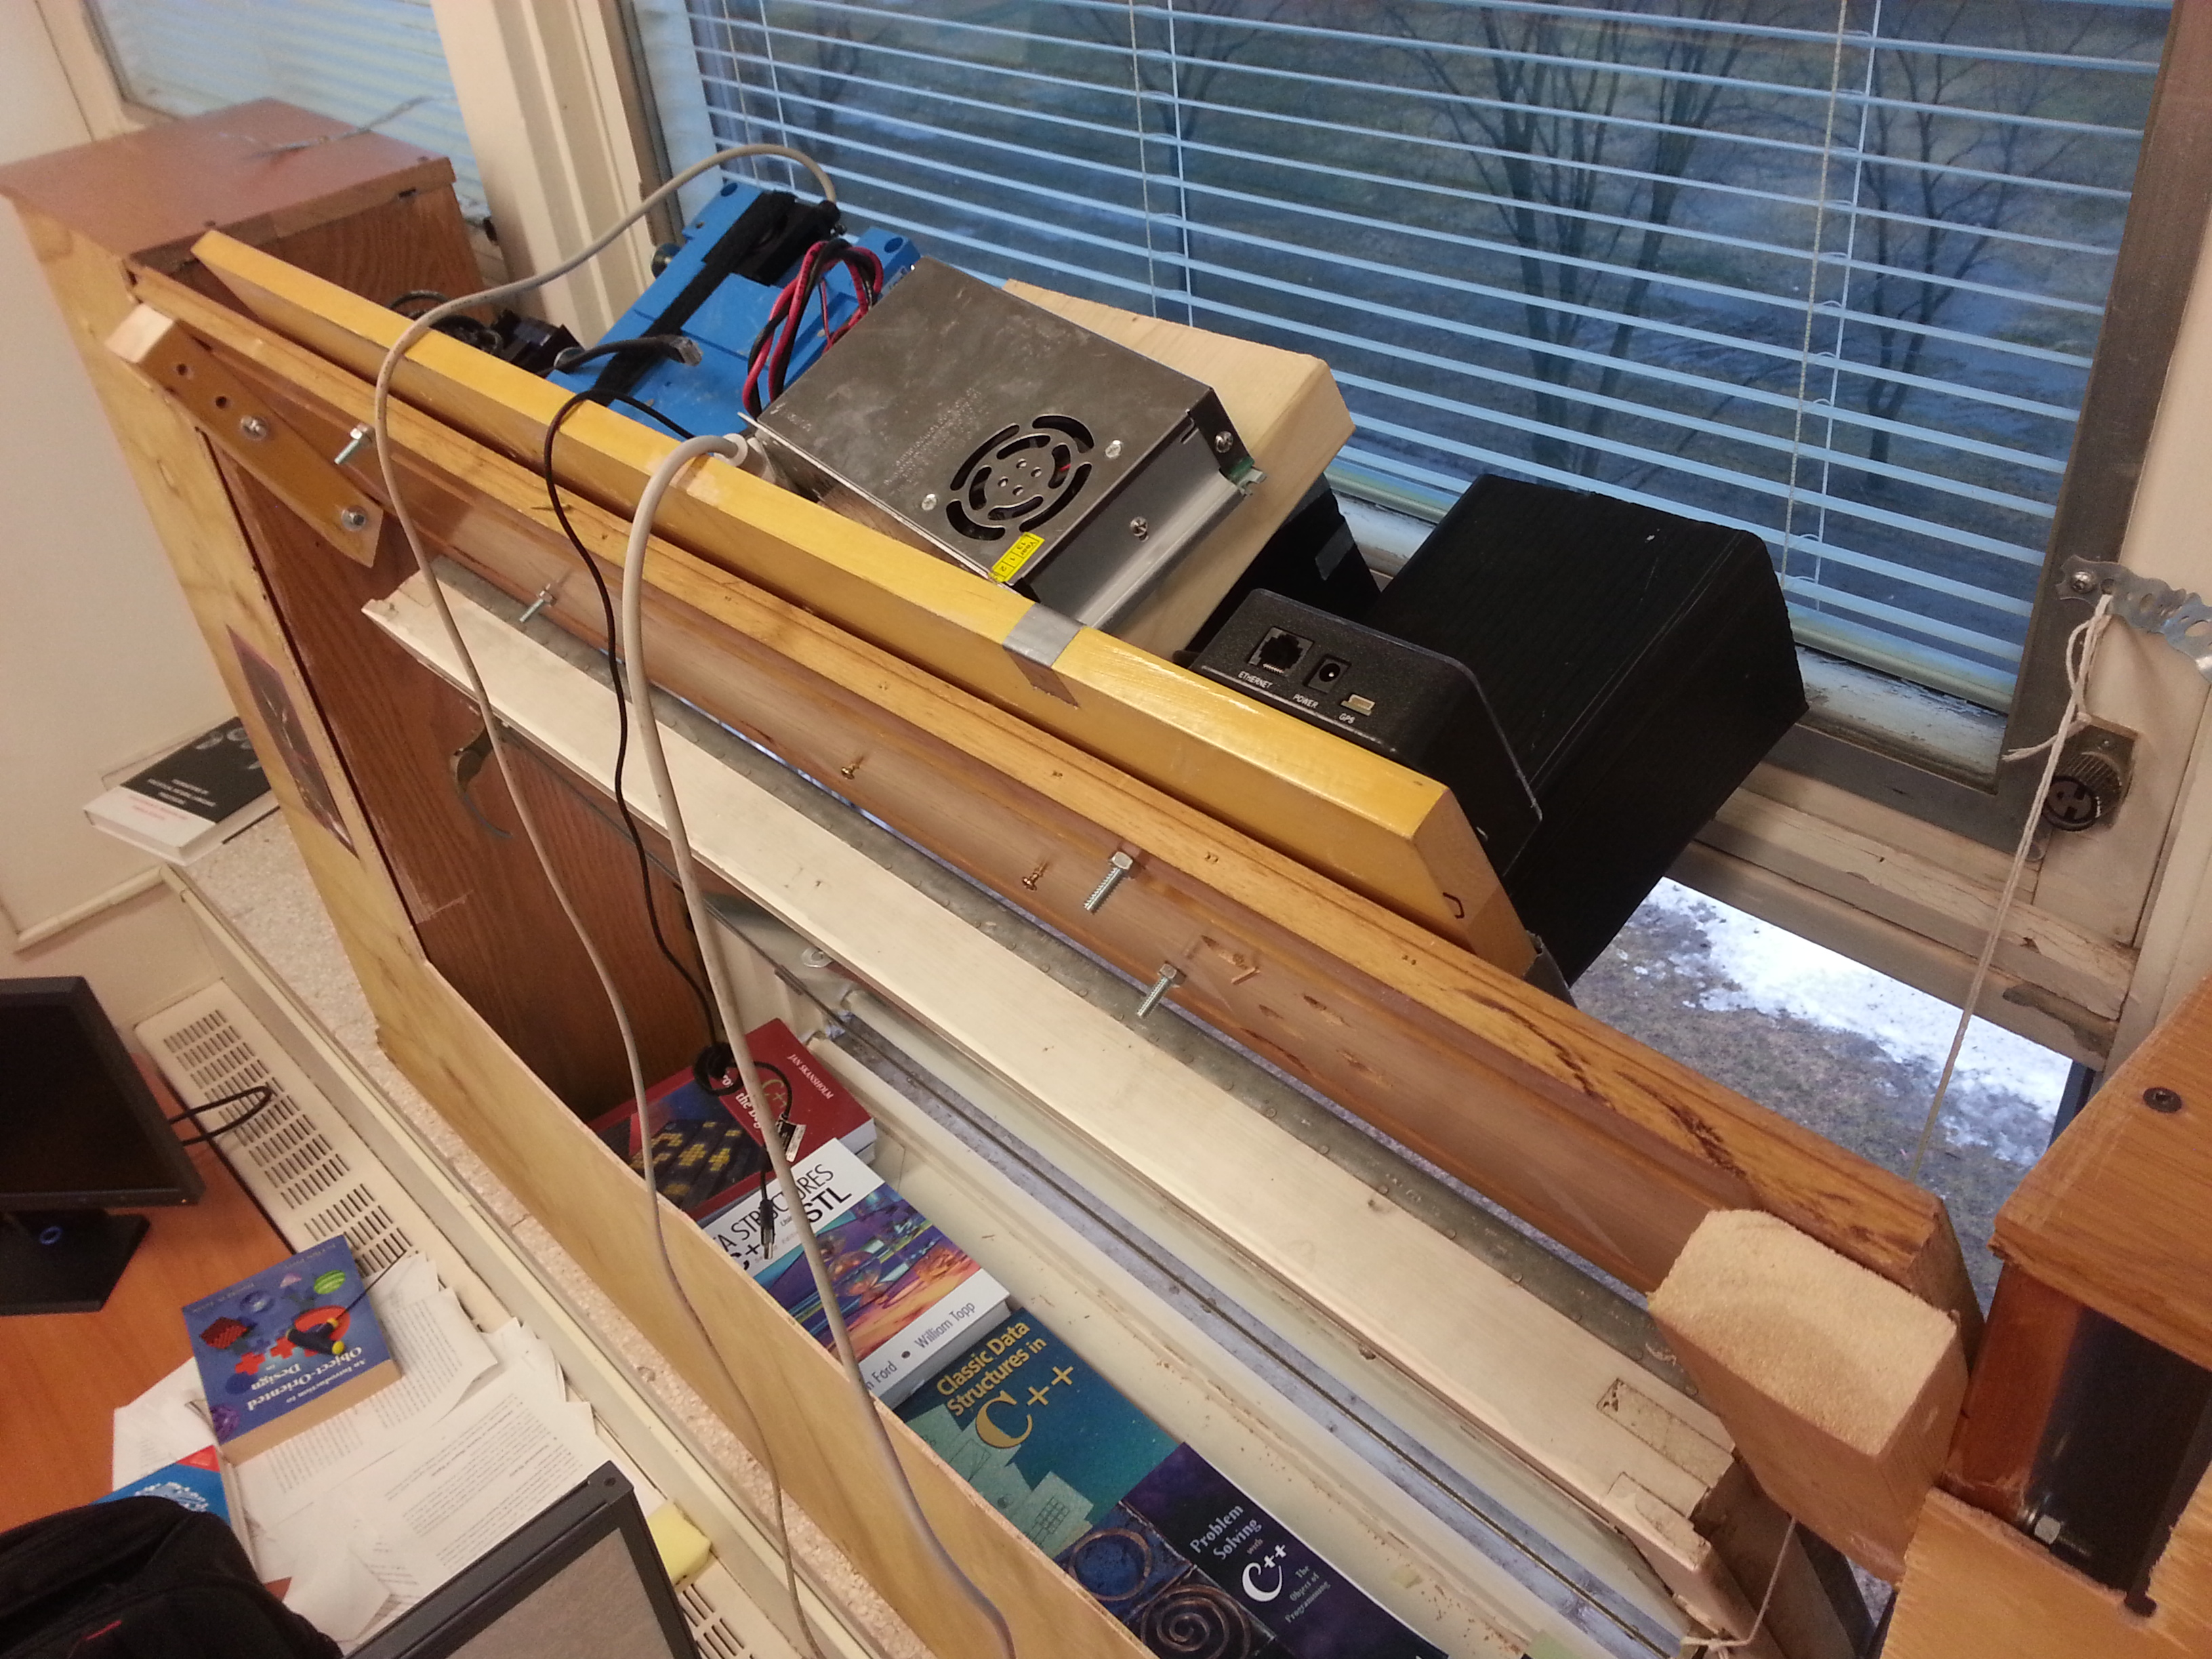
\includegraphics[width=0.9\linewidth]{./img/setup_diag.jpg}
    \caption{The experimental set-up}
    \label{fig:setup}
\end{figure}

Some notes to fill up the table:
\begin{itemize}
    \item LMS200
        \begin{itemize}
            \item See page 8. Range vs reflectivity
            \item See page 7. It is around 20cm at 20m
            \item Class 1, $\lambda=905 nm$
        \end{itemize}
    \item LMS151
        \begin{itemize}
            \item See page 25. Scanning range up to 50 m (164.04 ft) with $>$ 75\% object remission (18 m (59.06 ft) with 10\% object remission)
            \item See page 26. $distance(mm (in)) * 0.015 rad + 8 mm (0.31 in)$
        \end{itemize}
    \item Hokuyo
        \begin{itemize}
            \item 0.1 to 10m : $\pm$30mm,10 to 30m : $\pm$50mm(White Kent Sheet)
            \item See article : Spot size is 50 mm × 500 mm at sensor’s maximum distance of 30 m
            \item See page 6. Up to 3 echoes.
        \end{itemize}
    \item Velodyne
        \begin{itemize}
            \item See manual page 12. 1 to 70 meters... Datasheet says 80-100m...
            \item See page 23. The lasers project a well defined rectangular shaped spot that is approximately 4” wide by 2” tall at 100’ distance. The spot size at the source of the HDL-32 is approximately 1/2” wide by 1/4” tall, causing the angular divergence to be 2.79 milliradians.
            \item Time of flight
        \end{itemize}
\end{itemize}

Table~\ref{tab:lidars} show differents informations about the LiDARs. Note that all LiDARs use class 1 laser with a wavelength of \SI{905}{\nano\meter}.
\begin{table}[htbp]
    \centering
    \begin{tabularx}{\linewidth}{|X||X|X|X|}\hline
        Sensor              & Multi echo & Beam angle & Max dist     \\ \hline%\hline
        Velodyne HDL-32E    & no         & beam       & Stuff        \\ \hline
        Hokuyo UTM-30LX-EW  & yes        & 0.25d      & 30/60m       \\ \hline% Garantee and max
        SICK LMS151         & no         & 0.5d       & 50m          \\ \hline% 50 m (at >75 % reflectivity) / 18 m (at 10 % reflectivity)
        SICK LMS200         & no         & beam       & Stuff        \\ \hline
    \end{tabularx}
    \caption{LiDARs informations}\label{tab:lidars}
\end{table}
